\documentclass[pdftex]{scrartcl}
\usepackage{longtable}
\usepackage{graphicx}
\title{\umlToCdl~System Description \\ Version 1.0}
\author{J\"urgen Doser and Burkhart Wolff\footnote{This work is part of the EU-funced TrustCom Project
 \texttt{http://www.eu-trustcom.com/}}}
\date{}

\newcommand{\st}[1]{\texttt{<<#1>>}}
\newcommand{\xml}[1]{\texttt{<#1>} \ldots \texttt{</#1>}}
\newcommand{\umlToCdl}{\texttt{UML2CDL}}
\newcommand{\cdl}{\texttt{CDL}}

\begin{document}
\maketitle

\section{Introduction}
\umlToCdl\ converts a UML model into the XML-based \emph{Choreography
  Description Language} \cdl~\cite{cdl} describing the interaction of
distributed processes occuring in web-based services. Since \cdl\
can be compiled to BPEL4WS~\cite{bpel05,qiu05} which can be
interpreted by BPEL-engines directly, \umlToCdl\ is the front-end of a
tool-chain allowing for the abstract description of (some aspects of)
web-based services following the \emph{model-driven architecture}
(MDA) approach.

This system description serves several purposes:
\begin{enumerate}
\item We describe the principle format of the supported UML model
  (essentially consisting of a class diagram and a collection of
  associated activity graphs),
\item we describe the principles of the translation,
\item we add a list of known restictions and don't do's necessary for
  the practical handling of \umlToCdl, and
%\item we will outline some future extensions of our tool.
\end{enumerate}

\section{The Structure of input \umlToCdl\ Models}

A UML Model that can be processed by \umlToCdl\ must have the
following structure:
\begin{enumerate}
\item it must have a class model (the \emph{base model}), defining the
  information types, partners, roles and relationships,
\item a number of activity graphs may be associated to classes of this
  model, describing the actual choreographies,
%\item \ldots 
\end{enumerate}

\subsection{Example: SAC}

For the SAC example, the class model is given in
Figure~\ref{fig:SAC-class-model}. 

\begin{figure}
  \centering
  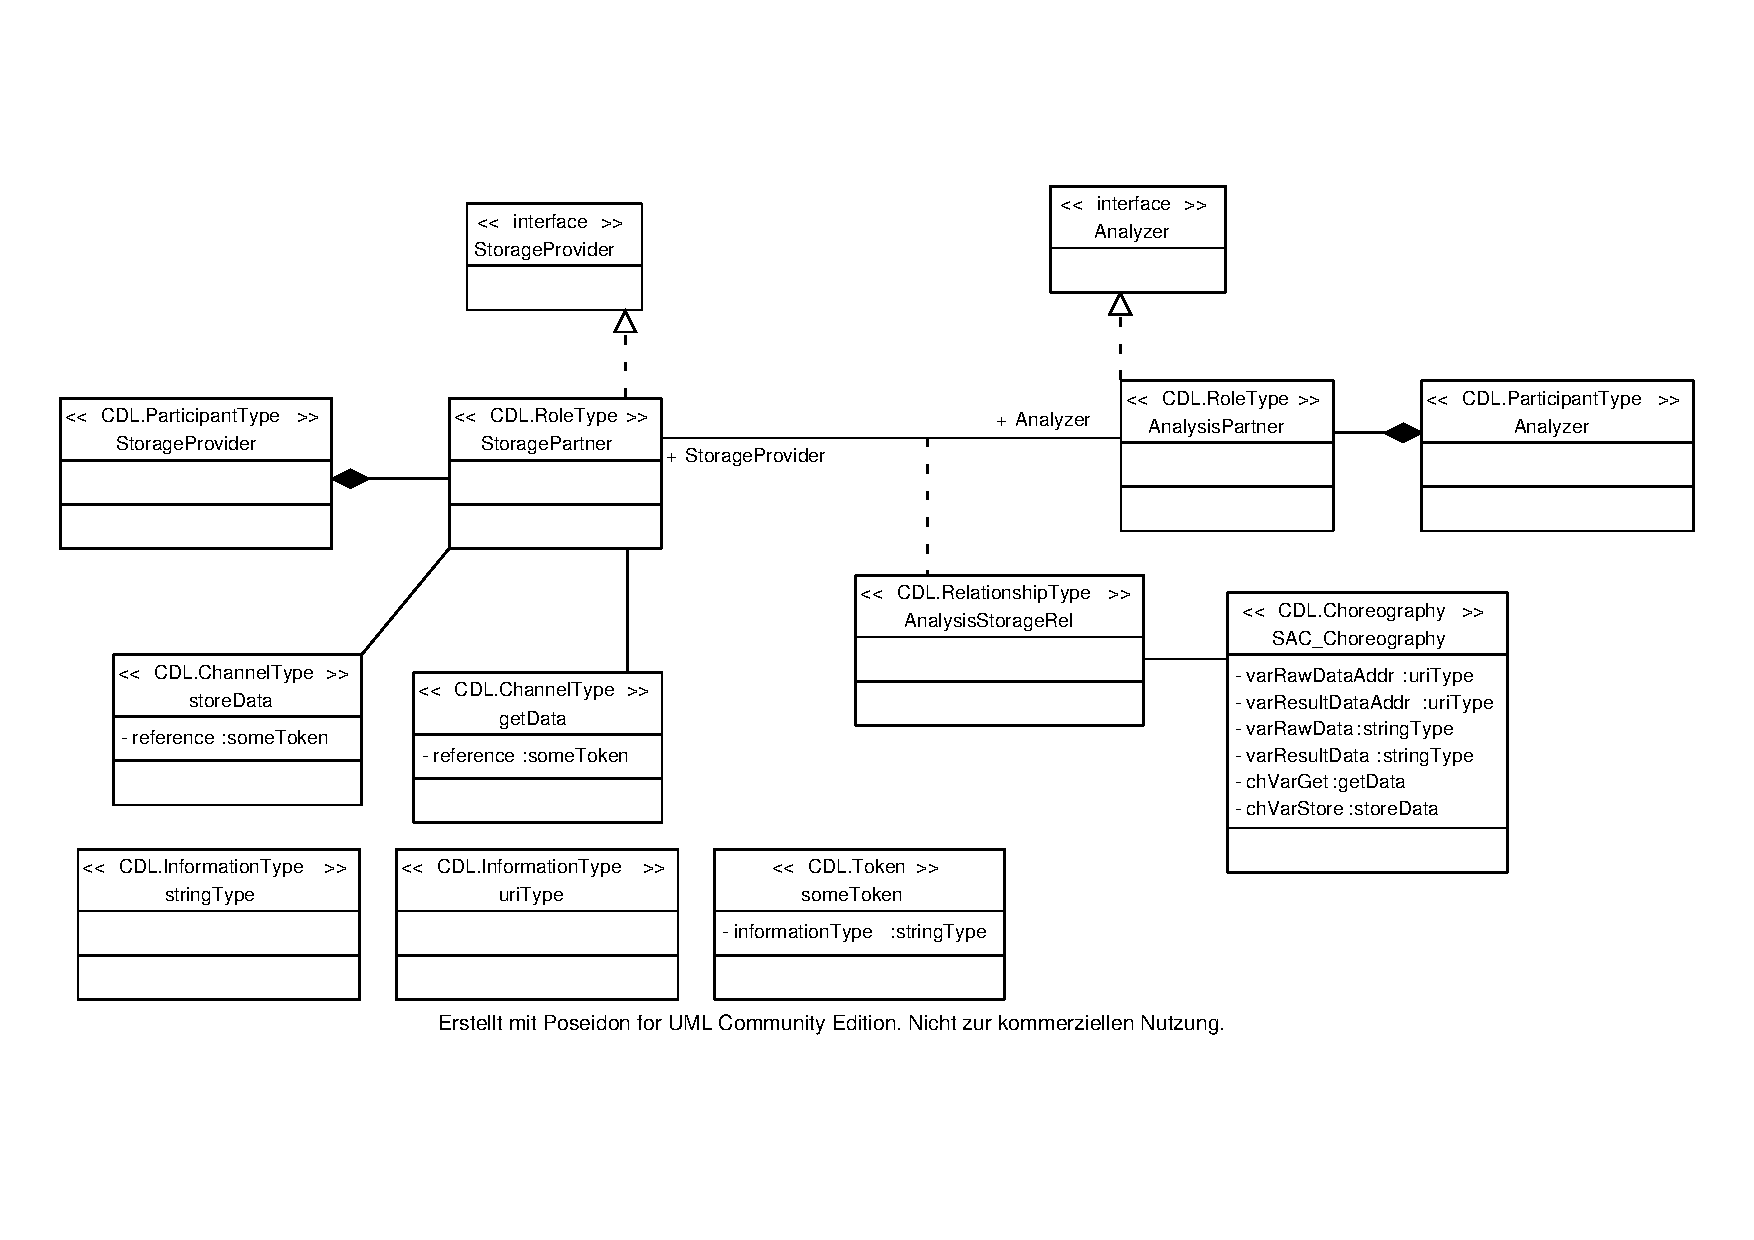
\includegraphics[scale=0.9,angle=90]{SAC_static_model.pdf}
  \caption{Class model for SAC}
  \label{fig:SAC-class-model}
\end{figure}

The actual dynamic behavior of the choreography is given in
Figure~\ref{fig:SAC-chor-model} 

\begin{figure}
  \centering
  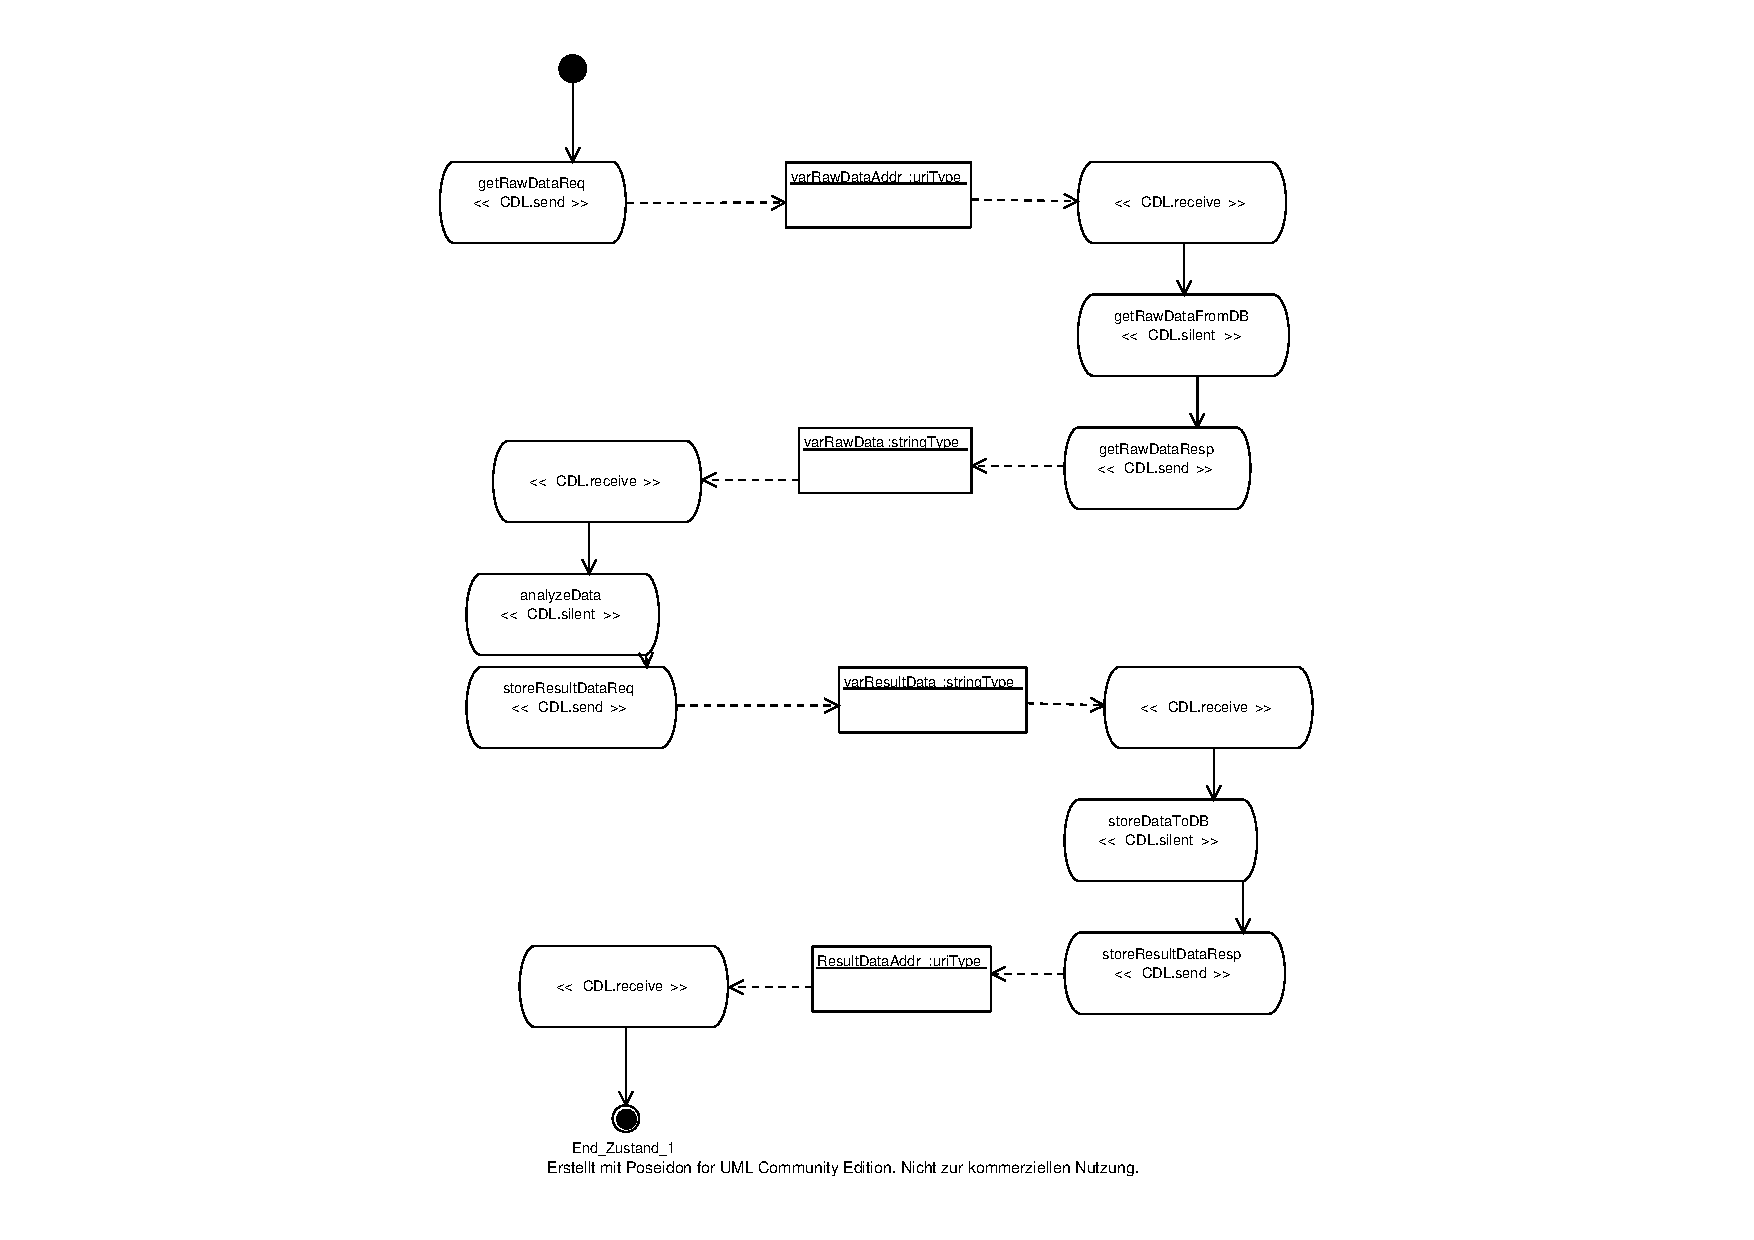
\includegraphics[trim=200 0 0 0]{SAC_chor_model.pdf}
  \caption{Choreography for SAC}
  \label{fig:SAC-chor-model}
\end{figure}


\subsection{Example: SAC2}

For the SAC2 example, the class model is given in
Figures~\ref{fig:SAC2-participants} and \ref{fig:SAC2-relationships}.
Note that the example is not yet fully modeled: the second parallel
activity is not complete. But it shows how to model parallel
activities. 

\begin{figure}
  \centering
  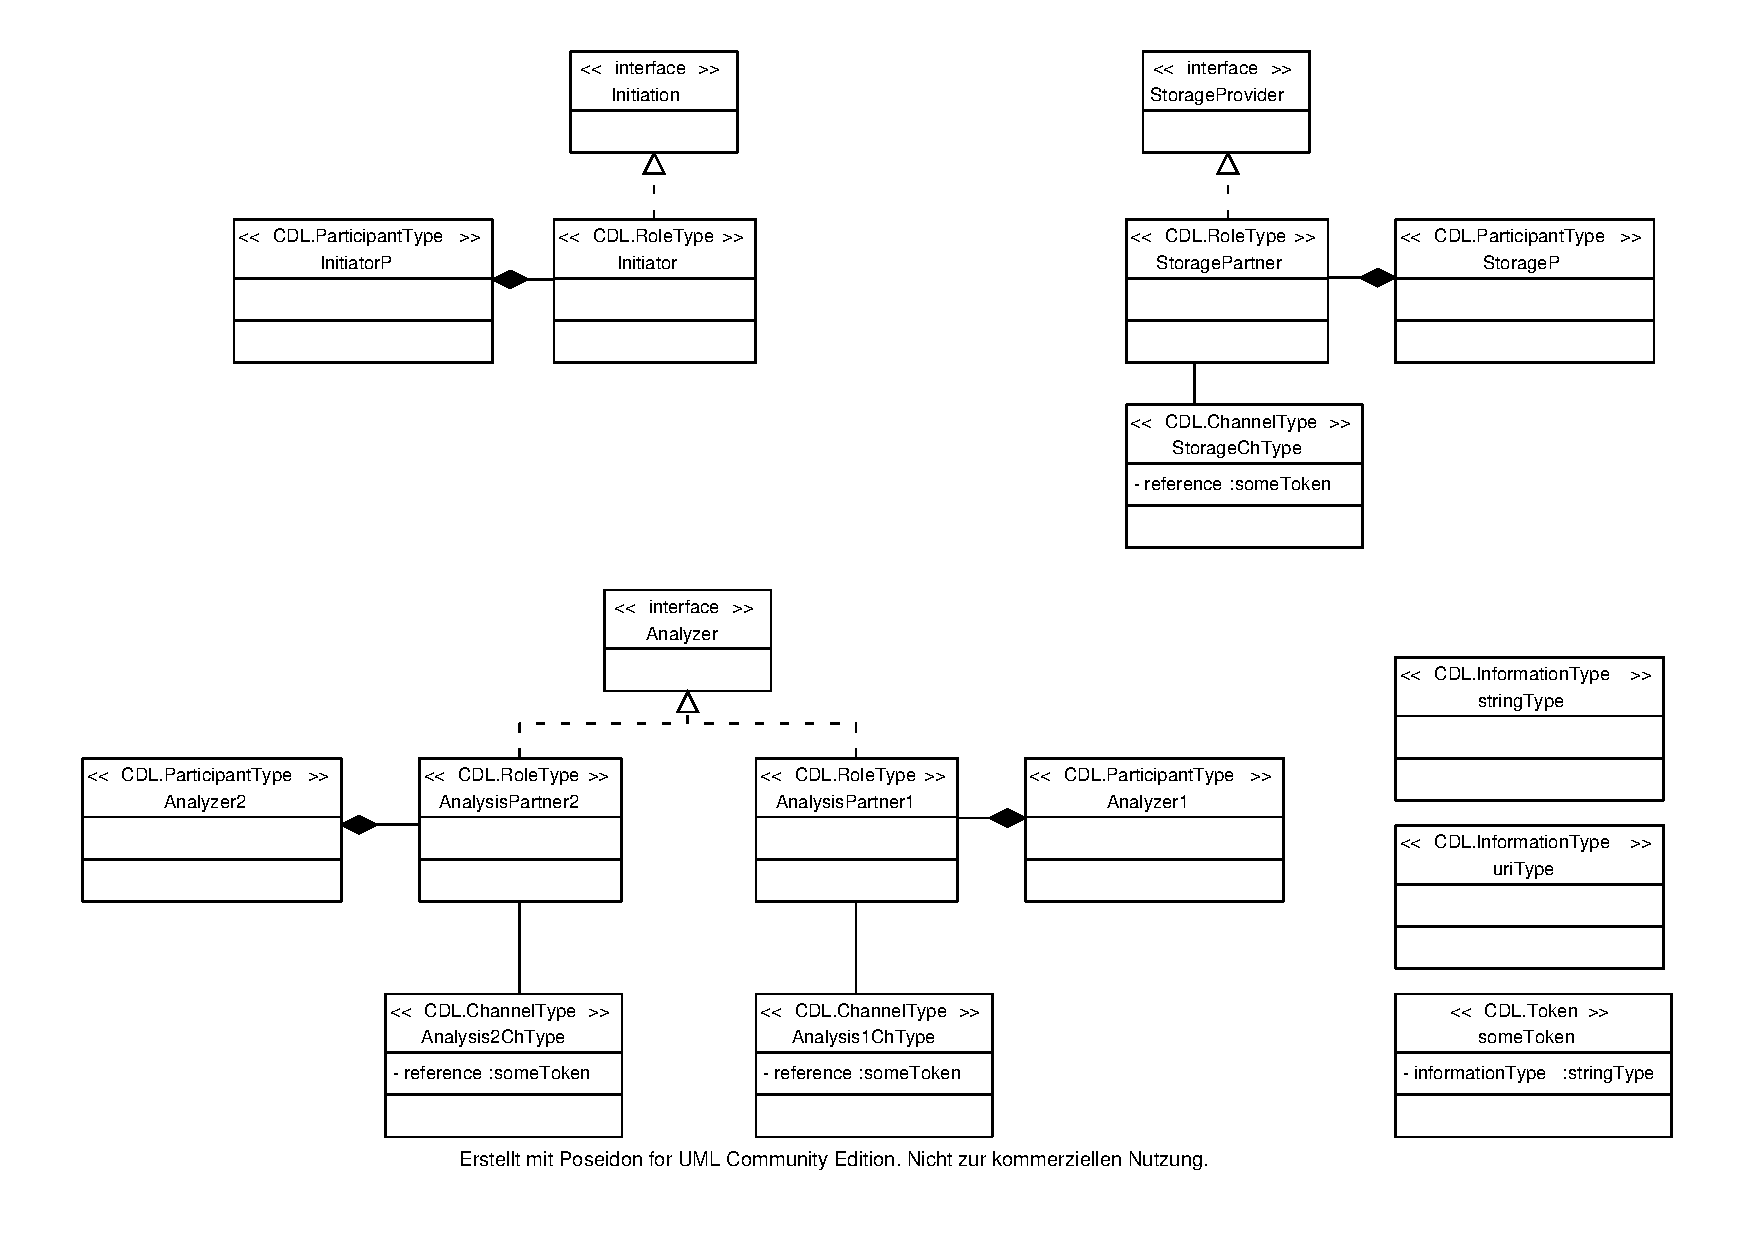
\includegraphics[scale=0.85,angle=90]{SAC2-participants.pdf}
  \caption{The participants in SAC2}
  \label{fig:SAC2-participants}
\end{figure}

\begin{figure}
  \centering
  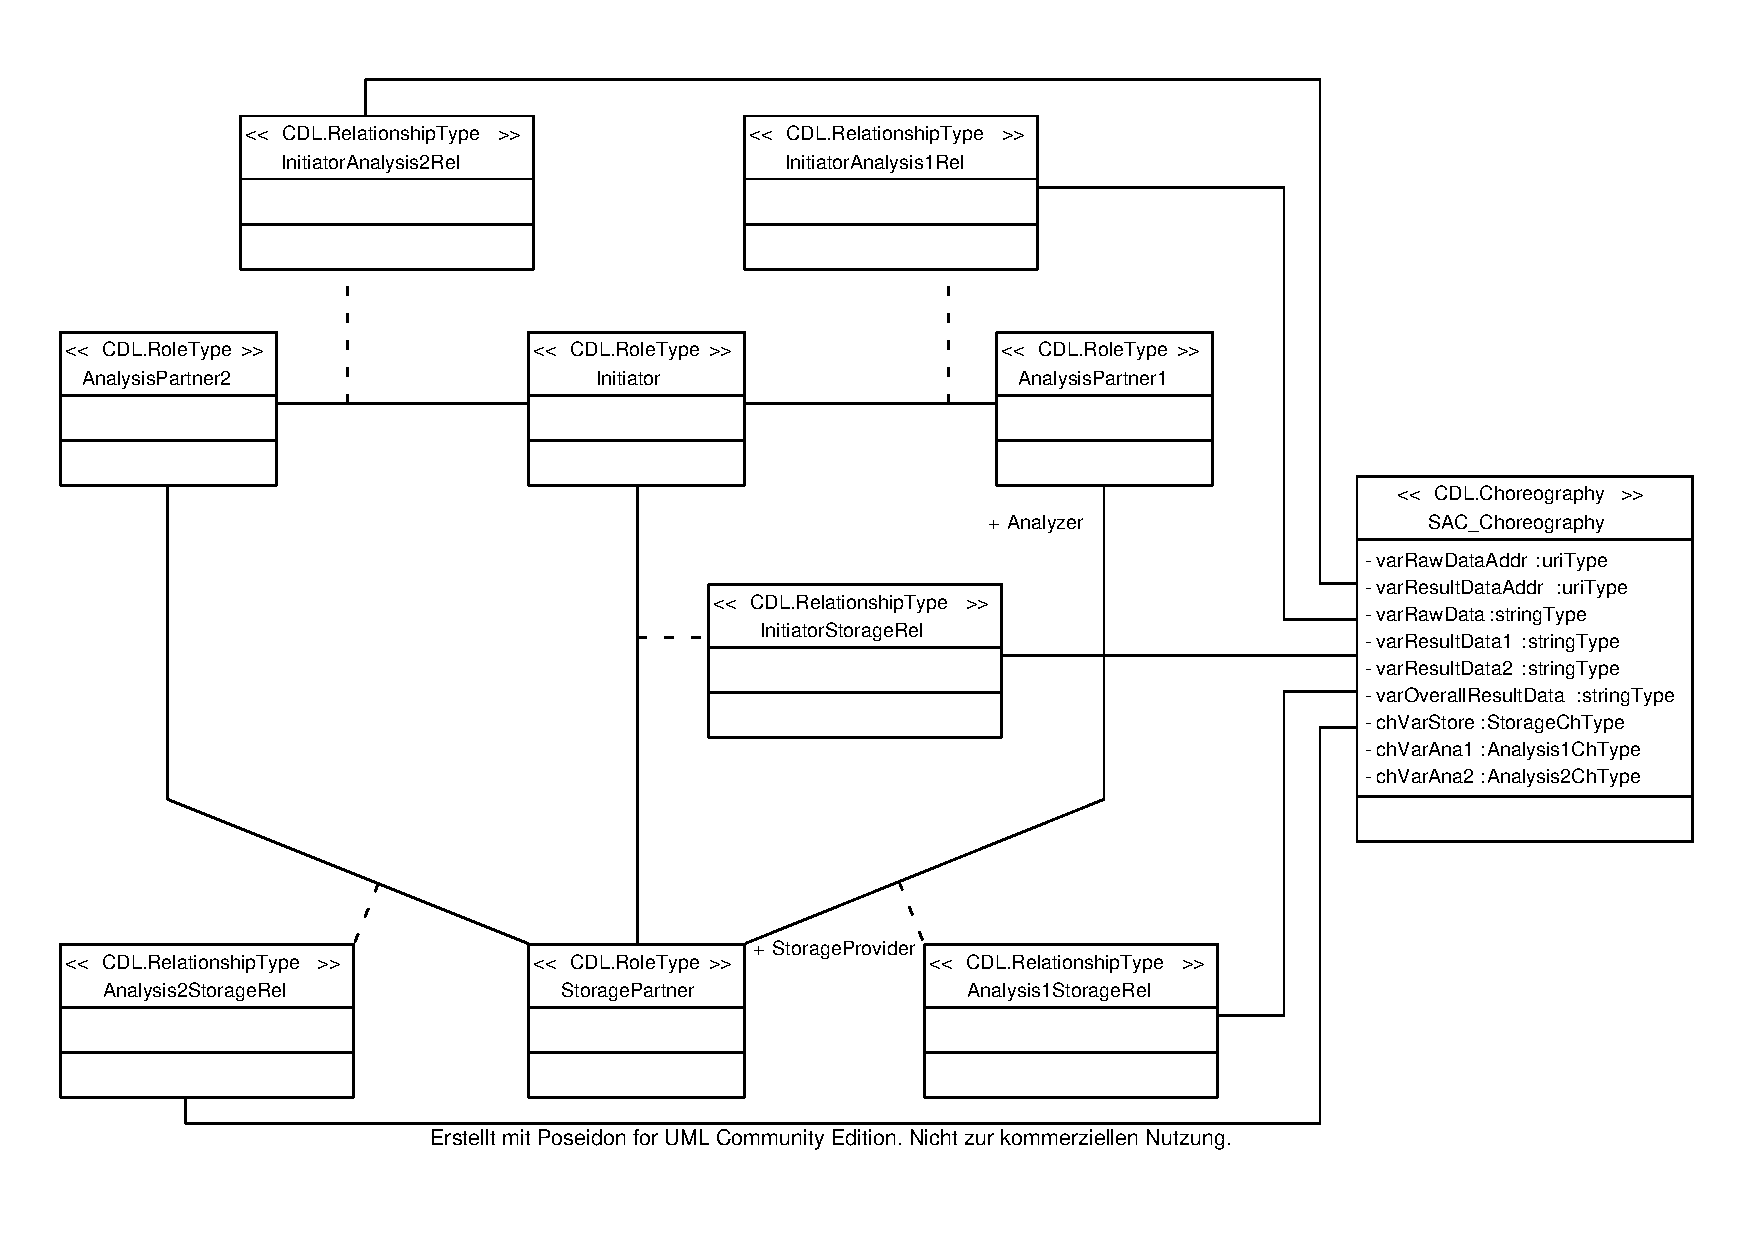
\includegraphics[scale=0.85,angle=90]{SAC2-relationships.pdf}
  \caption{the relationships in SAC2}
  \label{fig:SAC2-relationships}
\end{figure}

The actual dynamic behavior of the choreography is given in
Figure~\ref{fig:SAC2-chor-model} 

\begin{figure}
  \centering
  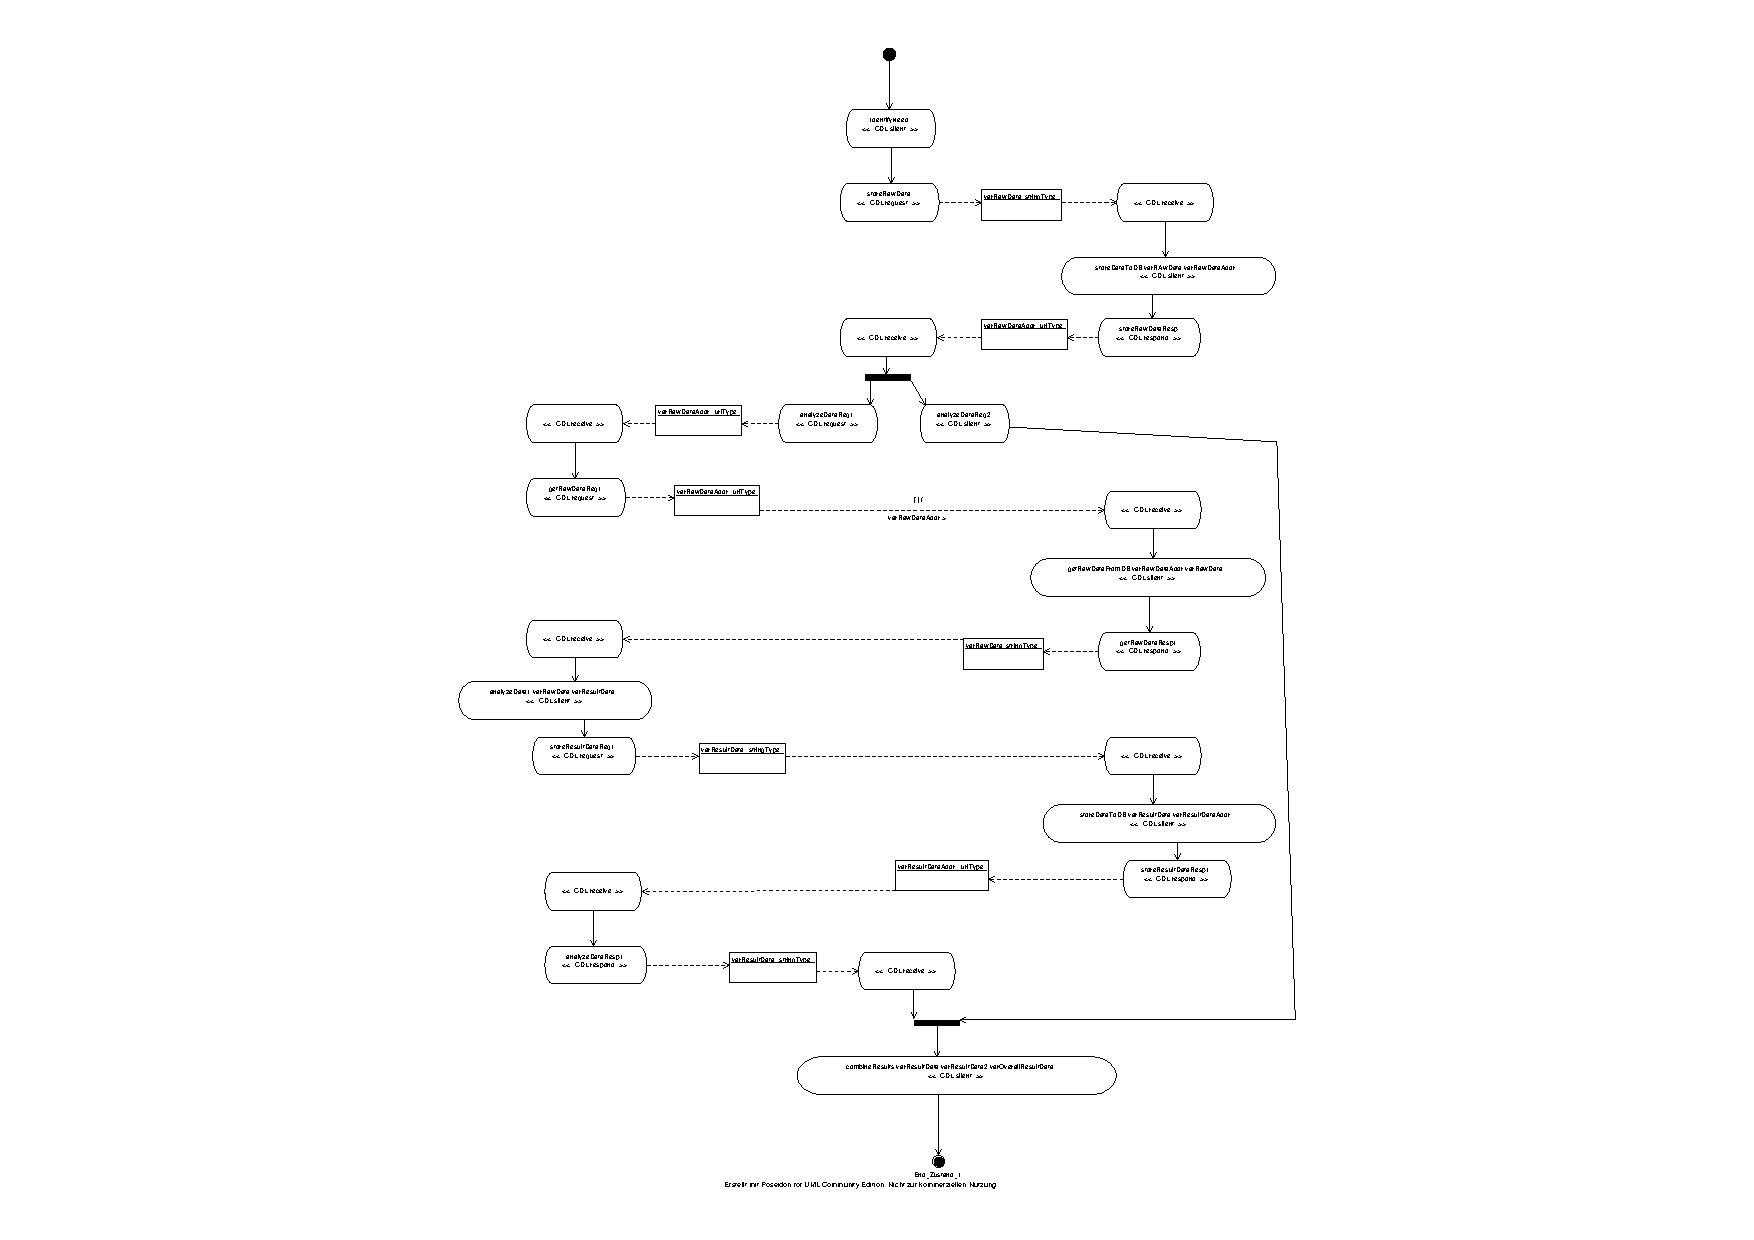
\includegraphics[trim=200 0 0 0]{SAC2-chor-model.pdf}
  \caption{Choreography for SAC2}
  \label{fig:SAC2-chor-model}
\end{figure}

\newpage

\section{The Translation}

\umlToCdl\ is implemented in SML and includes a particular package
called fxp~\cite{fxp} for the XML processing. SML is a functional
programming language with a strong type system supporting parametric
polymorphism, parameterized modules (functors), pattern matching and
higher-order functions. As such, it is particularly suited for
symbolic computations and the flexible construction of compilers.
Although developped internally with the SML implementation SML/NJ
110.52~\cite{njml}, \umlToCdl\ has been cross-compiled via the SML
compiler MLton\cite{mlton} to ANSI-C.  On this basis, an \texttt{.exe}
binary 
%as well as \texttt{.dll} libraries
has been generated to be used in the TrustCom system architecture on
Windows platforms using the cygwin environment.
\footnote{Acknowledgements to Achim Brucker who contributed to this
  part of our build process.}

\umlToCdl\ consists of three phases:
\begin{enumerate}
\item a generic XML-parser based on fxp,
\item a component converting the parsed XML-tree into 
      an abstract syntax for XMI following the UML 1.4
      standard (as supported by Poseidon 3.1, see below).
\item a component converting the XMI representation into
      \cdl.
\end{enumerate}

In the following, we focus on key elements of the translation of
the XMI into CDL.

\begin{longtable}{p{5cm}|p{4.5cm}|p{5.5cm}}
  \textbf{UML Model Element with Stereotype}& \textbf{WS-CDL Element} & 
  \textbf{Remark} \\\hline\hline
  Package            \st{CDL.Package}       & \xml{package}          &
  attribute \texttt{name} is taken from the name of the package, 
  attributes \texttt{author}, \texttt{version} and
  \texttt{targetNamespace} can be specified using tagged values
  \texttt{CDL.author}, \texttt{CDL.version} and
  \texttt{CDL.targetNamespace}  \\\hline 
  Class              \st{CDL.InformationType}  & \xml{informationType}  &
  %I'm not sure if we really have to model them explicitely, or if we
  %can derive them from the types of the attributes/variables in the
  %choreography. This is related to the question of how do we handle
  %tokens, and token locators.
  attribute \texttt{exceptionType} is taken from the tagged value
    \texttt{CDL.exceptionType}. The attribute \texttt{type}
    (resp. \texttt{element} is \emph{currently} taken from the tagged
    value \texttt{CDL.type} (resp. \texttt{CDL.element}).  We can
    discuss to use class attributes with names \texttt{type} or
    \texttt{element} instead, whose types corresponds to classes in
    another package describing the WSDL or some SML Schema.  
  \\\hline
  Class              \st{CDL.Token}            & \xml{token}
  & the information type of the token is given by the attribute with
  name \texttt{informationType}\\
  
  \\\hline
  Class              \st{CDL.ChannelType}      & \xml{channelType}
  & the role of a channel is given by an association, the reference
  type by the attribute with name \texttt{reference}. the
  \texttt{identity} and \texttt{passing} elements are currently not
  supported. 
  \\\hline
  Class              \st{CDL.RoleType}         & \xml{roleType}         &
  the behaviors of a roletype are specified using realisations of
  interfaces. \\\hline 
  AssociationClass   \st{CDL.RelationshipType} & \xml{relationshipType} &
  the roles in a relationship are given by the classes/roletypes
  connected to this association class\\\hline 
  Class              \st{CDL.ParticipantType}  & \xml{participantType}  &
  the roletypes of a participant type are specified using composite
  aggregations from the participant type to the role type\\\hline
  Class              \st{CDL.Choreography}     & \xml{choreography} &
  The attribute \texttt{complete}, \texttt{isolation}, \texttt{root},
  and \texttt{coordination}  can be specified using the tagged
  values \texttt{CDL.complete}, \texttt{CDL.isolation},
  \texttt{CDL.root} and \texttt{CDL.coordination}.  The variables
  (both informationtype and channeltype) used in the choreography are
  specified using attributes of the respective type. The roletypes of
  the variables are specified by the tagged value \texttt{CDL.roletypes}
  \\\hline
  Interface          ---                       & \xml{behaviour}
  & only when realised by a roletype (see above)
  \\\hline
  Activity           \st{CDL.silent}           & \xml{silent} & The
  partition to which the state belongs defines the roleType. The
  description of the silent actions is given by the body of the entry
  action, if the language of the entry action expression is either
  ``documentation'', ``reference'', or ``semantics'' (which are the
  possible description types in WS-CDL)
  \\\hline
  Activity           \st{CDL.noAction}         & \xml{noAction} & The
  partition to which the state belongs defines the roleType.
  \\\hline
  Activity           \st{CDL.request} of \st{CDL.respond}  & \xml{send}
  & see Objectflow below
  \\\hline
  Activity           \st{CDL.receive}          & \xml{receive}
  & see Objectflow below
  \\\hline
  ObjectFlow                               & \xml{exchange} & the
  connected action states are translated to send and receive
  activities, a sequence of such objectflows defines an
  \xml{interaction}. The name of the variable transfered in the
  exchange is given by the name of the objectflow state, the
  information type of the exchange is given by the type of the objectflow
  state. The action (request resp. response) is given by the stereotype of the send
  action -> \texttt{<<CDL.request>>} and \texttt{<<CDL.respond>>}. The
  relationshipTye, the channelVariable, and the operation for this
  interaction are given by tagged values, the fromRole and the toRole
  of the exchange are given by the partition of the send and receive
  states (the order depends on whether it is a request or a respond
  exchange). 
   \\ \hline
  successive activities                    & \xml{sequence} & 
  \\ \hline
  Fork Pseudostate                     & \xml{parallel} & all
  subsequent activities up to the matching join pseudostate \\\hline
\end{longtable}

Not every detail of the description above may be currently fully
implemented (see the remarks), but no big obstacle in implementing
them are expected. 

The following tables shows major elements that are currently not
implemented at all:

\begin{longtable}{p{5cm}|p{4.5cm}|p{5.5cm}}
  \textbf{UML Model Element with Stereotype}& \textbf{WS-CDL Element} & 
  \textbf{Remark} \\\hline\hline
  Activity           \st{CDL.perform}          & \xml{perform}          &
  \\\hline
  Choice Pseudostate  ---                  & \xml{choice} & \\\hline
\end{longtable}

Furthermore, it is as yet undecided, how to handle workunits and
tokenLocators. 
 
\section{Known Restrictions and Useful Workarounds}
A number of restrictions are imposed on \umlToCdl\ Version 1.0:
\begin{enumerate}
\item the XMI currently must be generated by \emph{Poseidon for UML
    3.1-0}, most likely the Community Edition. Support for
  Together Designer 2005 may be possible in the future.  Support for
  Together Control Center or other earlier versions of Borland
  Together is unlikely.
\item don't use cut-copy-paste when editing the diagrams: this may
  lead to sharings of model-elements and inconsistent XMI output of
  Poseidon.
\item since Poseidon 3.1-0 does unfortunately not support
  swimlanes/partitions in activity charts, we currently require to
  encode them by adding the tagged value \emph{partition} with
  a string containing its name.
\item the tool currently does almost no exception handling and input
  checking, so it requires some care to provide a model that is 
  sufficiently consistent to process it. 
\end{enumerate}

%\section{Conclusion}


\bibliography{trustcom} 
{\small
\sloppy
\bibliographystyle{abbrv}
}


\end{document}
